\chapter{态、测量与复矢量空间}

\lectureoverview{量子力学首先改变了我们对“态”的理解。我们首先分离出经典理论中态的模式与确定性更新，然后借助一个双结果自旋实验来揭示它的失败。数学上的回应是引入一个复矢量空间，并为其配备对偶矢量、内积、范数与正交性。}

\section{经典模式：态与更新}

从一个封闭系统开始，至少暂时将它与其他一切隔离开来。“\emph{系统}”一词在这里是原始概念：它指的是我们希望预测其历史的那个对象。“\emph{态}”则是在某一瞬间为了作出该预测而必须知道的一切。经典力学提供了一条将一个态更新为下一个态的定律。

对于最简单的抽象硬币，
\begin{equation}
  \mathcal S_{\mathrm{coin}}=\{H,T\}.
\end{equation}
一种可能的定律说，什么也不会发生：
\begin{equation}
  H\longmapsto H,
  \qquad
  T\longmapsto T.
\end{equation}
另一种定律则使两个态交替：
\begin{equation}
  H\longmapsto T,
  \qquad
  T\longmapsto H.
\end{equation}
这些例子虽然初等，却揭示了一个经典理论的架构：
\begin{equation}
  s(t)\longmapsto s(t+\Delta t).
\end{equation}
一旦\(s(t)\)已知，更新就是确定性的。

当态空间连续时，同样的模式依然成立。在一条直线上运动的粒子既需要位置也需要动量，
\begin{equation}
  s=(q,p),
\end{equation}
因此它的态空间是相平面。可能状态的数量变成了无穷多，方程也可以用拉格朗日量、哈密顿量与泊松括号的优雅语言来书写，但基本思想并未改变。某一时刻的态包含了预测另一时刻的态所需的信息。

\section{先抽象，后可视化}

经典运动相对容易想象，因为它的概念取自日常经验。当相关对象太小、速度太大，或者态空间的维数太高时，这种优势便消失了。没有人能真正在字面意义上想象电子的运动、四维时空或十维空间。这并不是初学者特有的缺陷。人类的视觉直觉是为日常的三维世界而建立的。

即使看似更简单的情形也暴露出这一局限。我们所谓的二维弯曲空间的图像，通常是一个嵌入三维空间中的曲面。一维直线则被想象为平面中的一个标记。图像悄悄引入了我们的视觉系统所熟悉的环境空间。

补救办法并不是把经典图像强加于陌生的物理之上，而是学习抽象结构，并让新的直觉从正确的操作中生长出来。三维坐标\((x,y,z)\)通过添加一个符号并扩展规则而变成四维坐标\((x,y,z,w)\)，而不是通过获得一种新的视觉器官。量子力学要求同样的训练。把它当作关于微小经典物体的奇怪力学模型，会一再导致错误的答案。

\begin{remark}
数学直觉仍然会发展起来。它只是不同于看见海洋中的波浪或普通空间中的箭头。代数之所以变得熟悉，是因为它的关系被一致地使用。
\end{remark}

\section{经典态空间与经典逻辑}

对于经典系统，态空间是一个集合。一个抽象骰子有
\begin{equation}
  \mathcal S_{\mathrm{die}}=\{1,2,3,4,5,6\}.
\end{equation}
一个真实的骰子有连续无穷多种取向，但这里所用的理想化骰子只有这六个标签。在一条直线上运动的粒子具有连续无穷集合
\begin{equation}
  \mathcal S_{\mathrm{particle}}
  =
  \{(q,p)\mid q,p\in\mathbb R\}.
\end{equation}
无论有限还是无限，每个经典态空间都是彼此不同的可能性的汇集。

关于系统的命题选取这些可能性中的一个子集。对于骰子，令
\begin{align}
  P_{\mathrm{odd}}&=\{1,3,5\},\\
  P_{\leq 3}&=\{1,2,3\}.
\end{align}
陈述“\emph{奇数且不大于三}”对应于它们的交集：
\begin{equation}
  P_{\mathrm{odd}}\cap P_{\leq 3}=\{1,3\}.
\end{equation}
包含性的陈述“\emph{奇数或不大于三}”对应于它们的并集：
\begin{equation}
  P_{\mathrm{odd}}\cup P_{\leq 3}
  =
  \{1,2,3,5\}.
\end{equation}
因此，经典合取与析取具有集合论形式
\begin{equation}
  P\wedge Q\longleftrightarrow P\cap Q,
  \qquad
  P\vee Q\longleftrightarrow P\cup Q.
\end{equation}
如果这些子集不重叠，就没有任何态能使两个命题同时为真。

这种逻辑与经典的态概念紧密相连。量子力学用另一种数学对象——矢量空间——取代了经典备选状态的集合。只有在适当的经典极限下，矢量空间描述才近似表现得像一组互斥的位形。在构造那个空间之前，我们需要一个使这种取代不可避免的实验。

\section{最简单的量子系统}

抽象硬币的量子对应物是一个双结果系统，称为\emph{量子比特}。其测量到的备选结果起初可以标记为正反两面，但数值标记更有用：
\begin{equation}
  \sigma\in\{+1,-1\}.
\end{equation}
将并行使用三种记号：
\begin{equation}
  H\longleftrightarrow \sigma=+1\longleftrightarrow\uparrow,
  \qquad
  T\longleftrightarrow \sigma=-1\longleftrightarrow\downarrow.
\end{equation}
起初箭头只是名称。尚未假定任何通常的几何矢量。

\begin{figure}[htbp]
  \centering
  \includegraphics[width=0.78\textwidth]{lecture_01_figure_02.png}
  \caption{黑板上引入了等价标记\(H/T\)、\(\sigma=\pm1\)以及上/下箭头。箭头起初只是记号，而不是经典模型。}
  \lectureframe{00:22:44}
\end{figure}

\begin{classroomqa}
\audiencequestion{正反两面与物理系统有什么关系？}
\lecturerresponse{除了提供两个熟悉的名称之外，没有任何关系。量子比特对于这一测量有两个可能结果；正反两面只是占位名称。之所以选择标记\(\pm1\)，是因为它们可以进入方程。}
\end{classroomqa}

\subsection{作为黑箱的装置}

实验需要第二个系统，即装置\(A\)。目前它是一个抽象黑箱，具有三个特征：
\begin{enumerate}
  \item 它具有空间取向，由\emph{此面朝上}标记；
  \item 它具有一个能够与量子比特相互作用的传感器；
  \item 它具有一个显示器，起初为空白，之后读数为\(+1\)或\(-1\)。
\end{enumerate}
探测器的细节被有意推迟。一个好的探测器由系统与其记录之间可靠的关系在操作上定义。相互作用发生时观察者不必正在观看；装置可以记录结果，之后再被读取。

假设显示器报告\(+1\)。将装置重置为空白状态，并在任何独立演化有时间起作用之前立即重复同一测量。一个忠实的探测器会再次报告\(+1\)。如果第一次结果是\(-1\)，立即重复同样继续报告\(-1\)：
\begin{equation}
\begin{aligned}
  +1&\longrightarrow +1\longrightarrow +1\longrightarrow\cdots,\\
  -1&\longrightarrow -1\longrightarrow -1\longrightarrow\cdots.
\end{aligned}
\end{equation}
因此，第一次测量可以被视为一种\emph{制备}。它使量子比特处于这样一种状态：立即重复同一测量会得到确定的结果。

这种可重复性不是可选的哲学附注。没有它，就没有操作性的方式来确认一次测量。一个有缺陷的装置可能无法重复其结果，但那样它就不是在进行这里所定义的理想测量。

\begin{classroomqa}
\audiencequestion{这已经是波函数坍缩了吗？}
\lecturerresponse{这种说法可以稍后引入。在这个阶段，操作性的陈述已经足够：一次测量产生一个结果，并制备一个状态，使得同一立即测量会重现该结果。给这个过程命名尚未解释它。}
\end{classroomqa}

\section{取向与经典指针的失败}

制备量子比特，使竖直放置的装置读数为\(+1\)。将装置转过\(180^\circ\)并重复测量。现在结果为\(-1\)。用倒置装置重复测量确认\(-1\)，而再次将装置转回竖直则恢复\(+1\)。

结果表明了真正的方向性。上/下记号并非完全任意：反转探测器会反转符号。人们很容易得出结论：量子比特只是一个很小的矢量，而探测器测量该矢量沿自身轴的分量。这种诱惑必须被检验，而不是被信任。

\begin{figure}[htbp]
  \centering
  \includegraphics[width=0.82\textwidth]{lecture_01_figure_03.png}
  \caption{黑板上的向上制备与不同取向的分析器。课堂上后来纠正了一个粉笔箭头的方向；在论证中只有分析器轴才重要。}
  \lectureframe{00:36:21}
\end{figure}

\subsection{侧向测量}

将探测器转过\(90^\circ\)。如果制备好的量子比特是一个通常的向上指针，那么它沿水平探测器轴的分量将为零：
\begin{equation}
  \hat{\mathbf x}\cdot\hat{\mathbf z}=0.
\end{equation}
量子装置从不报告零。每一次单独试验都报告\(+1\)或\(-1\)。

\begin{figure}[htbp]
  \centering
  \resizebox{\linewidth}{!}{%
  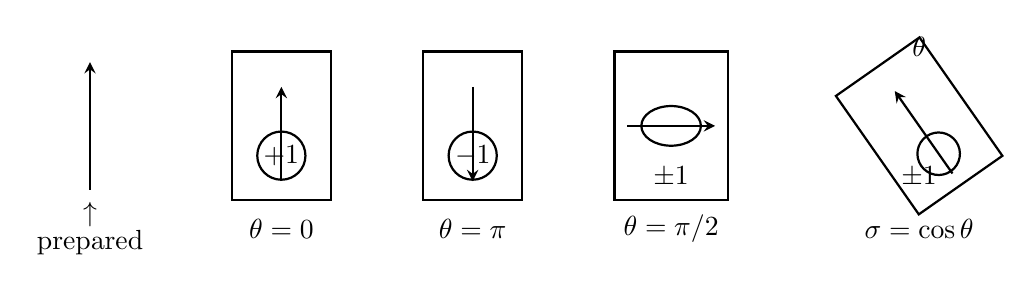
\begin{tikzpicture}[>=stealth,thick,scale=0.90]
    \draw[->] (0,0)--(0,1.8);
    \node at (0,-0.35) {\(\uparrow\)};
    \node at (0,-0.75) {prepared};

    \draw (2.0,-0.15) rectangle (3.4,1.95);
    \draw (2.7,0.48) circle (0.34);
    \draw[->] (2.7,0.12)--(2.7,1.45);
    \node at (2.7,0.48) {\(+1\)};
    \node at (2.7,-0.55) {\(\theta=0\)};

    \draw (4.7,-0.15) rectangle (6.1,1.95);
    \draw (5.4,0.48) circle (0.34);
    \draw[->] (5.4,1.45)--(5.4,0.12);
    \node at (5.4,0.48) {\(-1\)};
    \node at (5.4,-0.55) {\(\theta=\pi\)};

    \draw (7.4,-0.15) rectangle (9.0,1.95);
    \draw (8.2,0.90) ellipse (0.42 and 0.28);
    \draw[->] (7.58,0.90)--(8.82,0.90);
    \node at (8.2,0.18) {\(\pm1\)};
    \node at (8.2,-0.55) {\(\theta=\pi/2\)};

    \begin{scope}[shift={(11.7,0.90)},rotate=35]
      \draw (-0.72,-1.02) rectangle (0.72,1.02);
      \draw (0,-0.48) circle (0.30);
      \draw[->] (0,-0.82)--(0,0.60);
    \end{scope}
    \node at (11.7,0.18) {\(\pm1\)};
    \node at (11.7,-0.55) {\(\expect{\sigma}=\cos\theta\)};
    \node at (11.7,2.02) {\(\theta\)};
  \end{tikzpicture}
  }%
  \caption{分析器序列的重构。旋转改变统计，而从不改变单个结果的集合。}
\end{figure}

用竖直装置制备大量量子比特，保留结果为\(+1\)的那些。用侧向装置对每个保留的量子比特测量一次。一半试验给出\(+1\)，一半给出\(-1\)，系综平均为零：
\begin{equation}
  \expect{\sigma}_{\pi/2}=0.
\end{equation}
平均值类似于经典指针消失的水平分量，但单个记录并非如此。经典值\(0\)已被两个离散结果之间的统计平衡所取代。

\begin{classroomqa}
\audiencequestion{如果在侧向量子测量之后不丢弃同一个量子比特，而是保留它，会发生什么？}
\lecturerresponse{假设它第一次的侧向结果是\(+1\)。对同一个量子比特重复侧向测量，会一次又一次地得到\(+1\)。第一次侧向测量已经相对于侧向轴制备了它。要获得五五开的统计，必须在许多量子比特上重复整个制备与测量实验，而不是反复确认一个结果。}
\end{classroomqa}

\subsection{不相容的制备}

轴的顺序很重要。沿竖直方向制备\(+1\)，然后沿水平方向测量。第一个水平结果随机。一旦获得了一个水平结果，立即重复水平测量就是确定的。现在把探测器转回竖直轴。竖直结果又变得随机了。

用符号表示，其中\(M_z\)和\(M_x\)表示沿两个轴的测量，
\begin{equation}
\begin{aligned}
  M_z&:+1,\\
  M_x&:\pm1,\\
  M_x&:\text{same result},\\
  M_z&:\pm1.
\end{aligned}
\end{equation}
中间的\(x\)测量并非仅仅在保持原竖直态的同时揭示出一个水平分量。它制备了一个新态，而原来的竖直确定性已经消失。

\begin{classroomqa}
\audiencequestion{探测器记得第一个答案吗？它怎么能知道呈现给它的是同一个量子比特还是一个新的量子比特？}
\lecturerresponse{可重复性是被测量量子比特的性质，而不是探测器执行的隐藏记忆比较。测量之后，量子比特处于一种状态，使得对同一立即测量的回答相同。呈现一个以不同方式制备的量子比特，结果就取决于那个制备。跟踪正在测量的是哪个物理系统，是普通的实验室记录工作。}
\end{classroomqa}

\begin{classroomqa}
\audiencequestion{所以观察行为制备了那个特定的量子比特？}
\lecturerresponse{是的。一旦那次测量制备了该量子比特，同一测量就会给出相同答案，直到某种其他演化或不相容的测量介入。}
\end{classroomqa}

\section{任意旋转的分析器}

设探测器轴与系综被制备所沿的轴成角\(\theta\)。每次试验仍然给出
\begin{equation}
  \sigma=\pm1.
\end{equation}
相对频率随角度变化，使得平均值为
\begin{equation}
  \expect{\sigma}_{\theta}=\cos\theta.
  \label{eq:qml1-cosine-mean}
\end{equation}
极限情形为
\begin{align}
  \expect{\sigma}_{0}&=+1,\\
  \expect{\sigma}_{\pi/2}&=0,\\
  \expect{\sigma}_{\pi}&=-1.
\end{align}
在\(\theta=0\)附近，大多数结果是\(+1\)，偶尔出现\(-1\)。在\(\theta=\pi\)附近，大多数是\(-1\)，偶尔出现\(+1\)。

\begin{figure}[htbp]
  \centering
  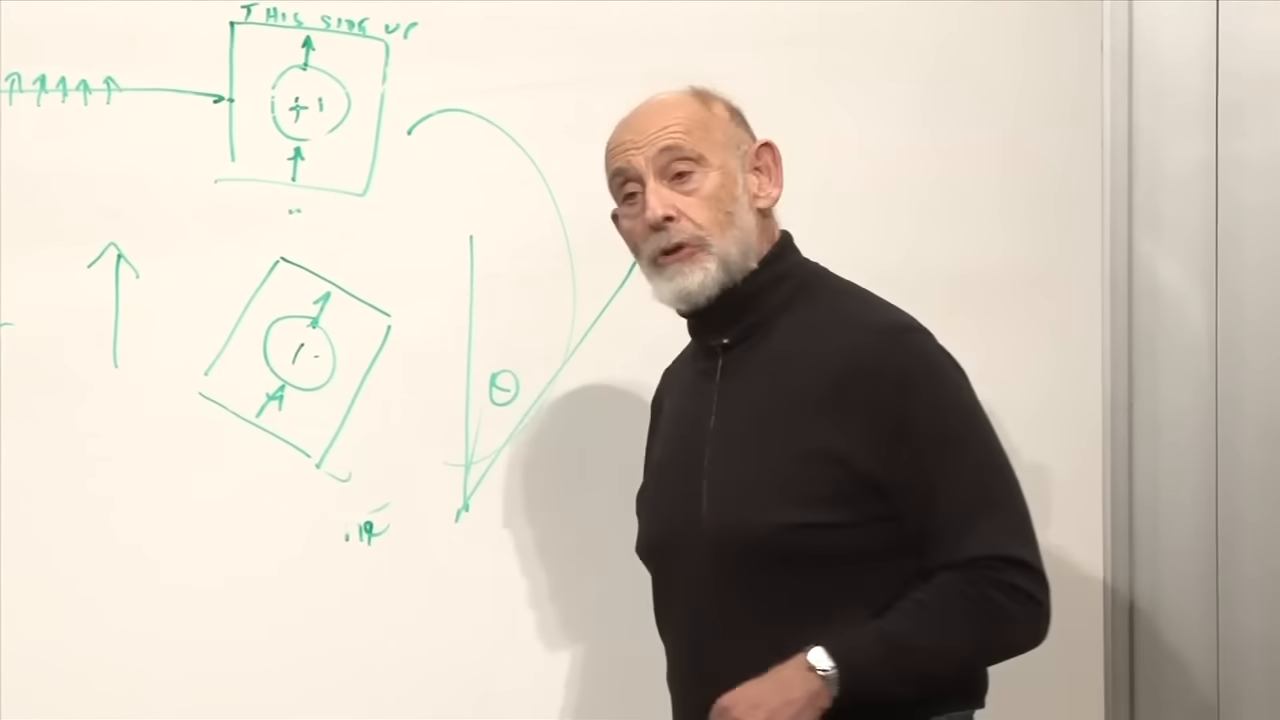
\includegraphics[width=0.82\textwidth]{lecture_01_figure_04.png}
  \caption{任意角度实验的实际板书：一个竖直制备的系综进入一个倾斜了\(\theta\)的分析器。}
  \lectureframe{00:48:55}
\end{figure}

光滑的类矢量量是系综平均值，而不是单个结果。如果\(p_+(\theta)\)和\(p_-(\theta)\)是两个概率，那么
\begin{equation}
  p_+ + p_-=1,
  \qquad
  p_+-p_-=\cos\theta.
\end{equation}
因此，
\begin{equation}
\begin{aligned}
  p_+(\theta)&=\frac{1+\cos\theta}{2}
  =\cos^2\frac{\theta}{2},\\
  p_-(\theta)&=\frac{1-\cos\theta}{2}
  =\sin^2\frac{\theta}{2}.
\end{aligned}
  \label{eq:qml1-half-angle-probabilities}
\end{equation}
\editorialnote{讲座陈述了两个结果及其平均值\(\cos\theta\)。方程~\eqref{eq:qml1-half-angle-probabilities}是这些陈述的直接代数推论，并使隐含的频率规律变得明确。}

\begin{classroomqa}
\audiencequestion{一个未制备的量子比特集合也会显示\(\cos\theta\)平均值吗？}
\lecturerresponse{在未极化集合中没有选择任何特定方向，所以其平均值为零。\(\theta\)依赖性指的是首先沿确定轴制备的系综。}
\end{classroomqa}

\begin{classroomqa}
\audiencequestion{如果量子比特没有中间动力学，为什么还需要整个系综？}
\lecturerresponse{对一个量子比特的第一次倾斜测量给出一个样本。对同一个量子比特的每一次立即重复都只是确认那个样本。独立试验需要全同制备的量子比特，每个都用倾斜分析器测量一次。}
\end{classroomqa}

\begin{classroomqa}
\audiencequestion{在正号和负号的序列中，是否存在模式或高阶关联？}
\lecturerresponse{对于这个实验，各次试验被视为独立且不相关。它们的单次试验概率依赖于\(\theta\)，但并未断言任何额外的排序模式。}
\end{classroomqa}

\subsection{被理想化了什么}

目前，仪器被当作一个经典物体，具有连续可调的方向和离散的读数。这种\emph{系统}与\emph{探测器}之间的划分是暂时的。探测器本身就是一个物理系统，最终必须服从量子力学。完整的描述将把系统和仪器一起处理，但那需要尚未具备的机制。

\begin{classroomqa}
\audiencequestion{探测器本身是否也只是另一个二态系统？}
\lecturerresponse{它具有物理状态，最终必须被纳入量子描述之中。目前我们保留一种操作性的区分：量子比特是被量子力学描述的对象，而定向探测器则提供稳定的经典记录。以后必须把这一组合系统作为相互作用的量子系统来分析。}
\end{classroomqa}

\begin{classroomqa}
\audiencequestion{改变探测器绕以旋转的轴，是否会引入比这里所示的单一角度更多的结构？}
\lecturerresponse{是的，完整的三维图景更为丰富。单平面内的旋转是其中最简单的切片，并且与即将给出的更完整处理相一致。}
\end{classroomqa}

\begin{classroomqa}
\audiencequestion{探测器能否返回介于\(-1\)与\(+1\)之间的连续值？}
\lecturerresponse{它的取向连续变化，但每次理想量子比特读出仍为\(+1\)或\(-1\)。连续性体现在取向变化时的概率和平均值中，而不体现在单个结果中。}
\end{classroomqa}

\section{指针与抽象矢量}

现在暂时把实验事实与数学分开。物理空间中的普通箭头将被称为\emph{指针}。数学矢量则更为一般：它是矢量空间的一个元素，不必指向普通空间中的任何方向。

\begin{definition}
复矢量空间\(V\)是一组矢量的集合，其中定义了矢量加法以及用复标量进行的乘法，并满足通常的线性规则。特别地，对于\(u,v,w\in V\)和\(a,b\in\mathbb C\)，
\begin{align}
  u+v&=v+u,\\
  (u+v)+w&=u+(v+w),\\
  a(u+v)&=au+av,\\
  (a+b)u&=au+bu,\\
  (ab)u&=a(bu),\\
  1u&=u.
\end{align}
存在零矢量\(0\)，并且对每个\(u\)都存在加法逆元\(-u\)。
\end{definition}

课堂讨论最初只强调运算和封闭性：
\begin{equation}
\begin{aligned}
  u,v\in V&\Longrightarrow u+v\in V,\\
  a\in\mathbb C,\ u\in V&\Longrightarrow au\in V.
\end{aligned}
\end{equation}
随后应提问补充了零矢量和交换律。其余熟悉的公理明确陈述了在引入具体列矢量模型时已经使用的内容。

实数构成\(\mathbb R\)上的一维矢量空间。复数构成\(\mathbb C\)上的一维矢量空间，以及\(\mathbb R\)上的二维矢量空间。复值函数\(\psi(x)\)也构成复矢量空间，因为
\begin{equation}
  (\psi+\phi)(x)=\psi(x)+\phi(x),
  \qquad
  (z\psi)(x)=z\psi(x).
\end{equation}
这个函数空间的例子以后将成为核心，但有限列矢量使结构更容易先被看清。

\begin{classroomqa}
\audiencequestion{矢量与矢量空间之间的区别是什么？}
\lecturerresponse{矢量是一个元素。矢量空间是所有这类元素的集合，连同将它们相加并用标量相乘的规则，正如一个数是一个对象，而数系是带有运算的集合。}
\end{classroomqa}

\section{二分量复列矢量}

用狄拉克符号把抽象矢量写为\(\ket{\alpha}\)。一个具体表示为
\begin{equation}
  \ket{\alpha}
  \longleftrightarrow
  \begin{pmatrix}
    \alpha_1\\
    \alpha_2
  \end{pmatrix},
  \qquad
  \alpha_1,\alpha_2\in\mathbb C.
\end{equation}
如果
\begin{equation}
  \ket{\beta}
  \longleftrightarrow
  \begin{pmatrix}
    \beta_1\\
    \beta_2
  \end{pmatrix},
\end{equation}
那么加法和标量乘法按分量定义：
\begin{align}
  \ket{\alpha}+\ket{\beta}
  &\longleftrightarrow
  \begin{pmatrix}
    \alpha_1+\beta_1\\
    \alpha_2+\beta_2
  \end{pmatrix},\\
  z\ket{\alpha}
  &\longleftrightarrow
  \begin{pmatrix}
    z\alpha_1\\
    z\alpha_2
  \end{pmatrix},
  \qquad z\in\mathbb C.
\end{align}

\begin{figure}[htbp]
  \centering
  \includegraphics[width=0.88\textwidth]{lecture_01_figure_05.png}
  \caption{两个复列矢量相加以及用复标量乘列矢量的分量规则。}
  \lectureframe{01:14:28}
\end{figure}

零矢量是
\begin{equation}
  \ket{0}
  =
  \begin{pmatrix}
    0\\
    0
  \end{pmatrix},
  \qquad
  \ket{\alpha}+\ket{0}=\ket{\alpha}.
\end{equation}
长度为三的列矢量构成另一个矢量空间，任意固定长度也类似。二分量列矢量不能与三分量列矢量相加，因为二者属于不同的空间，且没有按分量关联它们的规则。

\begin{classroomqa}
\audiencequestion{列矢量是矩阵吗？}
\lecturerresponse{在一般术语中，它是只有一列的矩阵。在本课程中，\emph{矩阵}一词通常指方阵，而单列数组将称为列矢量。这一区别是术语上的，而不是关于代数的分歧。}
\end{classroomqa}

\begin{classroomqa}
\audiencequestion{矢量加法的顺序重要吗？}
\lecturerresponse{不重要。按分量相加从复数继承了交换性：
\[
  \ket{\alpha}+\ket{\beta}
  =
  \ket{\beta}+\ket{\alpha}.
\]
这是矢量空间公理之一。}
\end{classroomqa}

\section{对偶矢量：左矢与右矢}

对于每个右矢\(\ket{A}\)，对偶空间中都有一个对应的矢量，写作\(\bra{A}\)。从右矢到左矢的映射是加性的，但会对复标量取复共轭：
\begin{align}
  \ket{A}+\ket{B}
  &\longleftrightarrow
  \bra{A}+\bra{B},\\
  z\ket{A}
  &\longleftrightarrow
  z^*\bra{A}.
  \label{eq:qml1-antilinear-dual}
\end{align}
第二条规则是本质性的复数特征。标量倍的右矢的对偶，要乘以该标量的复共轭。

\begin{figure}[htbp]
  \centering
  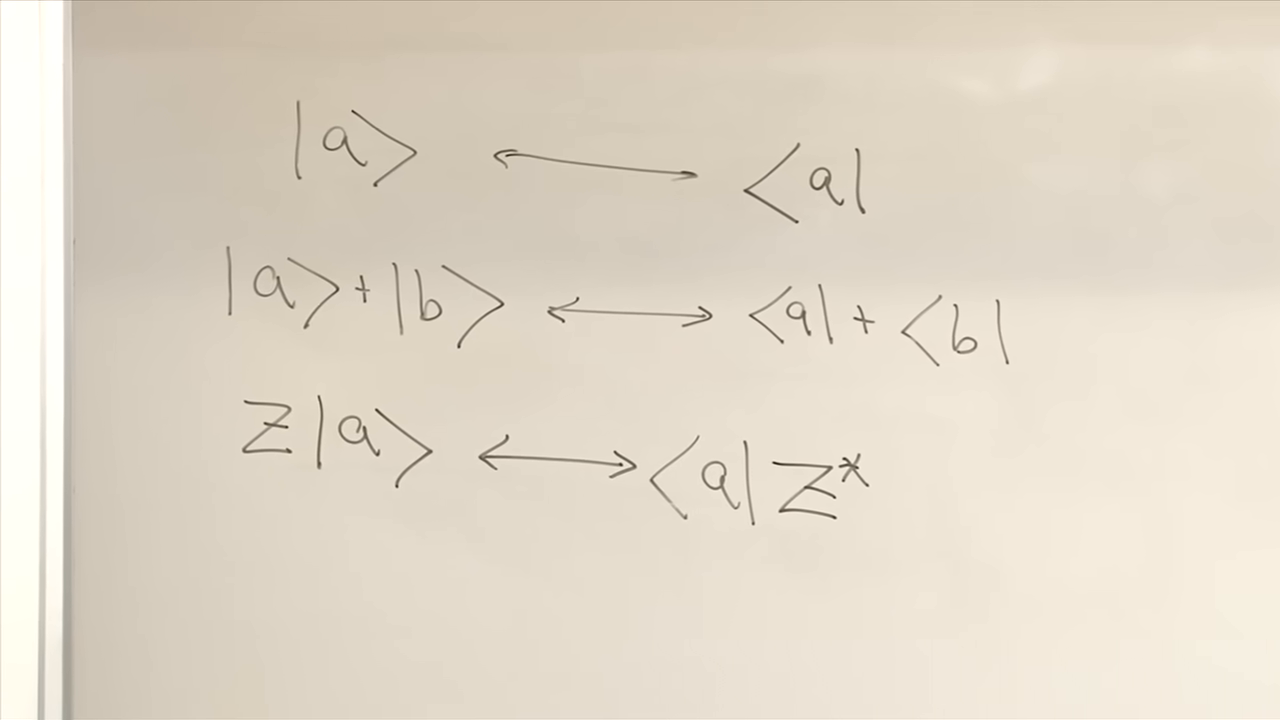
\includegraphics[width=0.86\textwidth]{lecture_01_figure_06.png}
  \caption{右矢到左矢的对应关系及其两条规则：和映射为和，而标量乘法取复共轭。}
  \lectureframe{01:23:15}
\end{figure}

对于二分量实现，
\begin{equation}
  \ket{\alpha}
  =
  \begin{pmatrix}
    \alpha_1\\
    \alpha_2
  \end{pmatrix}
  \qquad\Longrightarrow\qquad
  \bra{\alpha}
  =
  \begin{pmatrix}
    \alpha_1^*&\alpha_2^*
  \end{pmatrix}.
  \label{eq:qml1-bra-from-ket}
\end{equation}
复共轭实现了对偶对应，而行向量记号使两类对象在视觉上保持区分。方程~\eqref{eq:qml1-bra-from-ket}也直接验证了方程~\eqref{eq:qml1-antilinear-dual}。

\section{内积}

给定\(\ket{\alpha}\)和\(\ket{\beta}\)，将\(\beta\)对应的左矢与右矢\(\alpha\)结合：
\begin{equation}
  \braket{\beta}{\alpha}
  =
  \begin{pmatrix}
    \beta_1^*&\beta_2^*
  \end{pmatrix}
  \begin{pmatrix}
    \alpha_1\\
    \alpha_2
  \end{pmatrix}
  =
  \beta_1^*\alpha_1+\beta_2^*\alpha_2.
  \label{eq:qml1-inner-product}
\end{equation}
\emph{bracket}一词正是由\emph{bra}和\emph{ket}拼合而成。这是点积的复数类比：将对应分量相乘并相加，其中左矢一侧取复共轭。

\begin{figure}[htbp]
  \centering
  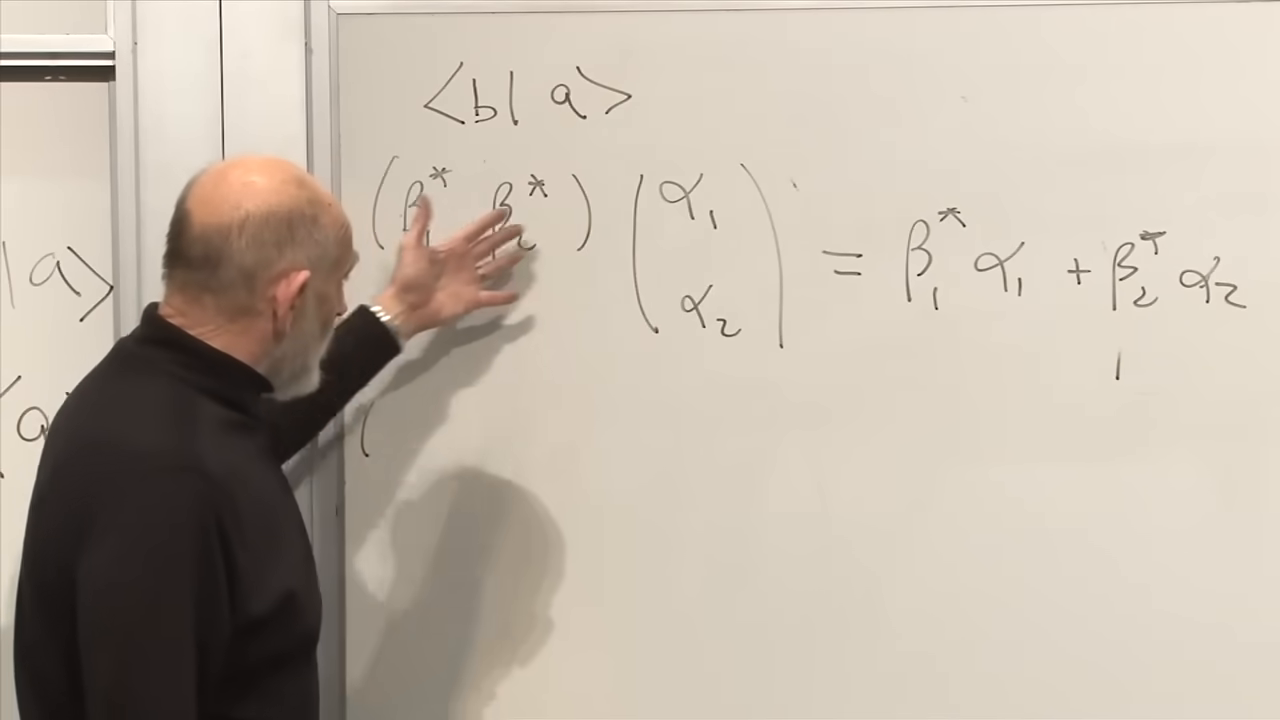
\includegraphics[width=0.88\textwidth]{lecture_01_figure_07.png}
  \caption{黑板上将内积\(\braket{\beta}{\alpha}\)计算为\(\beta_1^*\alpha_1+\beta_2^*\alpha_2\)。}
  \lectureframe{01:31:25}
\end{figure}

交换两个向量得到
\begin{equation}
  \braket{\alpha}{\beta}
  =
  \alpha_1^*\beta_1+\alpha_2^*\beta_2
  =
  \braket{\beta}{\alpha}^{*}.
  \label{eq:qml1-conjugate-symmetry}
\end{equation}
因此顺序一般是有影响的，但仅相差一个复共轭。

\begin{classroomqa}
\audiencequestion{能否不 conjugate 一侧而定义复向量的乘积？}
\lecturerresponse{可以构造这样的双线性表达式，但此时一个向量与自身的乘积未必为实数或正数。这种结构对量子力学并不有用。取共轭的、即 Hermitian 的内积给出了所需的范数与概率结构。}
\end{classroomqa}

\subsection{范数与正定性}

在方程~\eqref{eq:qml1-inner-product}中令\(\beta=\alpha\)：
\begin{equation}
  \braket{\alpha}{\alpha}
  =
  \alpha_1^*\alpha_1+\alpha_2^*\alpha_2
  =
  |\alpha_1|^2+|\alpha_2|^2.
  \label{eq:qml1-norm-square}
\end{equation}
这个数等于自身的复共轭，因此是实数。它非负，且仅对零向量为零。长度定义为
\begin{equation}
  \|\alpha\|
  =
  \sqrt{\braket{\alpha}{\alpha}}.
\end{equation}
因此复分量给出一个普通的非负实长度。

\begin{figure}[htbp]
  \centering
  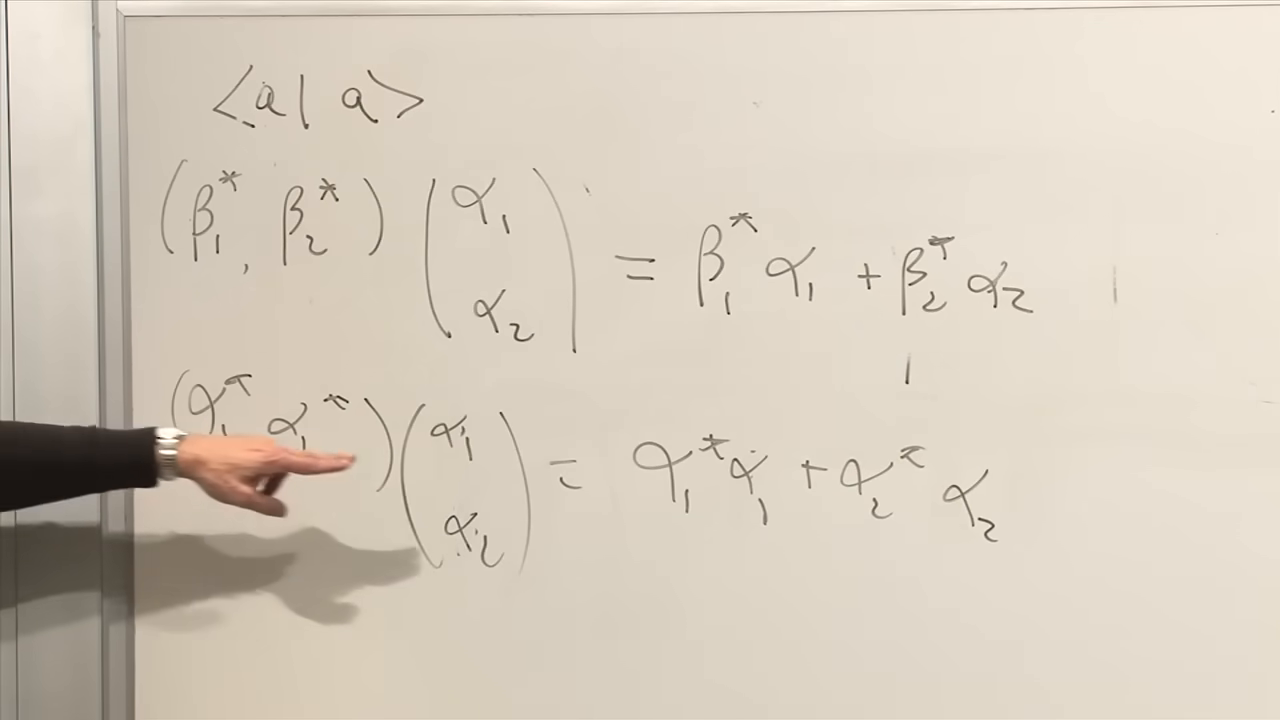
\includegraphics[width=0.88\textwidth]{lecture_01_figure_08.png}
  \caption{黑板上的自内积：\(\braket{\alpha}{\alpha}=|\alpha_1|^2+|\alpha_2|^2\)，即范数的平方。}
  \lectureframe{01:34:40}
\end{figure}

\section{正交性与维数}

当两个向量的内积为零时，它们正交：
\begin{equation}
  \braket{\beta}{\alpha}=0.
  \label{eq:qml1-orthogonality}
\end{equation}
共轭对称性使这一关系与顺序无关：
\begin{equation}
  \braket{\beta}{\alpha}=0
  \quad\Longrightarrow\quad
  \braket{\alpha}{\beta}
  =
  \braket{\beta}{\alpha}^{*}
  =0.
\end{equation}

在二分量空间中，最简单的正交对是
\begin{equation}
  \ket{e_1}
  =
  \begin{pmatrix}
    1\\
    0
  \end{pmatrix},
  \qquad
  \ket{e_2}
  =
  \begin{pmatrix}
    0\\
    1
  \end{pmatrix},
  \qquad
  \braket{e_1}{e_2}=0.
  \label{eq:qml1-standard-basis}
\end{equation}

\begin{figure}[htbp]
  \centering
  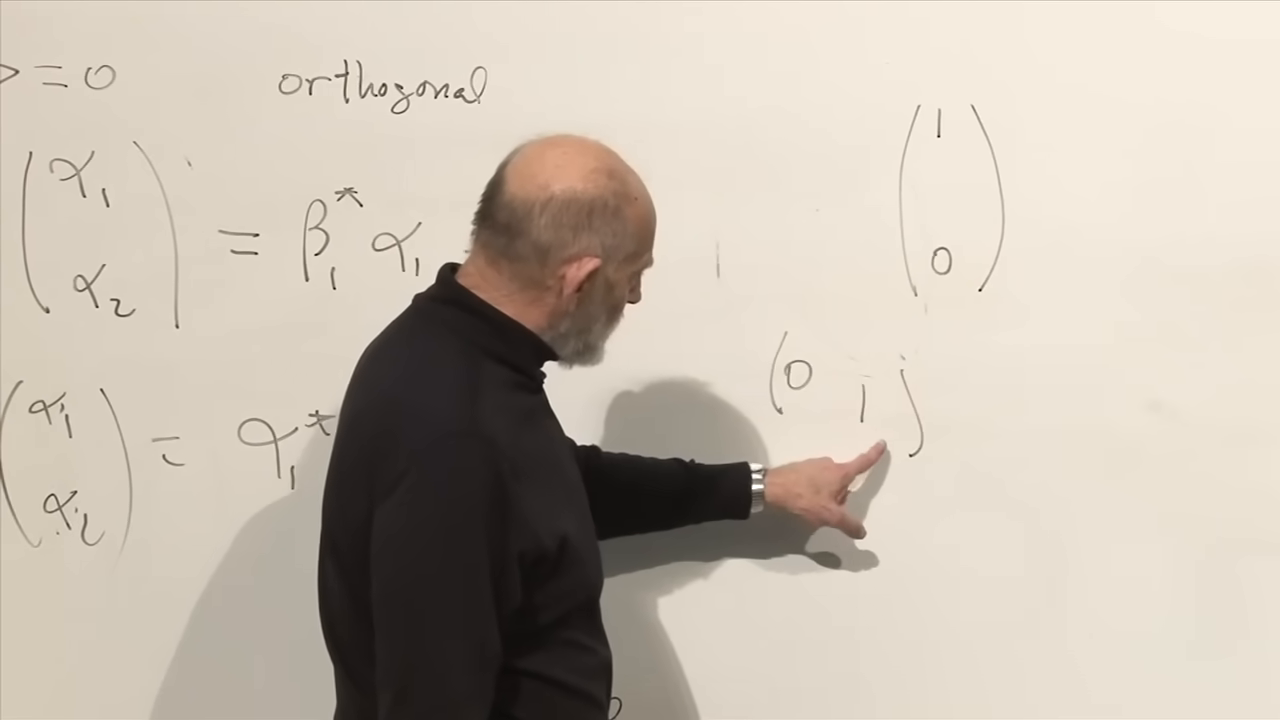
\includegraphics[width=0.88\textwidth]{lecture_01_figure_09.png}
  \caption{黑板上构造了标准正交列\((1,0)^{\mathsf T}\)和\((0,1)^{\mathsf T}\)。}
  \lectureframe{01:39:50}
\end{figure}

维数可以刻画为相互正交的非零向量的最大数目。在二维空间中，这样的向量可以有两个，但不可能有第三个。为具体看出这一点，令
\begin{equation}
  \ket{v}
  =
  \begin{pmatrix}
    v_1\\
    v_2
  \end{pmatrix}
\end{equation}
与方程~\eqref{eq:qml1-standard-basis}中的两个向量都正交。于是
\begin{equation}
  \braket{e_1}{v}=v_1=0,
  \qquad
  \braket{e_2}{v}=v_2=0,
\end{equation}
所以\(\ket{v}=\ket{0}\)。不存在与两者都正交的第三个非零向量。

\begin{classroomqa}
\audiencequestion{零向量不是与每个向量都正交，从而多提供一个吗？}
\lecturerresponse{是的，这正是定义必须说\emph{非零}的相互正交向量的原因。零向量不携带独立的方向，在计算维数时被排除。}
\end{classroomqa}

\begin{remark}
在列向量表示中，维数等于分量的数目。正交性的定义更为抽象，并不依赖于已经选定了坐标。
\end{remark}

\section{黑板上的进一步问题}

\begin{classroomqa}
\audiencequestion{同样的结构是否适用于函数构成的向量空间？}
\lecturerresponse{是的。函数可以看作一个列向量，其分量由连续指标\(\psi(x)\)标记。加法与数乘都是逐点进行的。相应的内积将变为积分而非有限求和；这一构造将在后面展开。}
\end{classroomqa}

\begin{classroomqa}
\audiencequestion{用左矢乘以右矢会产生一个矩阵吗？}
\lecturerresponse{是的。内积\(\bra{\beta}\ket{\alpha}\)将一个行向量与一个列向量缩并，产生一个数。交换顺序，\(\ket{\alpha}\bra{\beta}\)，产生一个外积，即一个方阵。内积与外积都将变得重要。}
\end{classroomqa}

\begin{classroomqa}
\audiencequestion{测量是真的影响了量子比特，而不只是揭示它吗？}
\lecturerresponse{是的。沿新轴进行的第一次测量制备了一个新态，这就是为什么重复该测量会确认答案，而回到旧轴则恢复不确定性。这种不可避免的扰动将量子实验与理想化的经典测量区分开来，后者原则上可以做得任意轻柔。}
\end{classroomqa}

\section{构造的两个部分}

现在，我们有了两个尚未连接起来的部分。实验部分说：
\begin{enumerate}
  \item 理想的量子比特测量只有\(\pm1\)两种结果；
  \item 重复进行同一个即时测量会确认该结果；
  \item 改变探测器的轴会改变测量所制备的状态；
  \item 对于一个已制备的系综，倾斜\(\theta\)的分析仪给出的平均值为\(\cos\theta\)。
\end{enumerate}
数学部分说：
\begin{enumerate}
  \item 量子态将由矢量而非经典点来表示；
  \item 相关的矢量构成一个复矢量空间；
  \item 右矢有对偶的左矢，而左矢在复标度下反线性地作用；
  \item 厄米内积定义了长度、正交性和维数。
\end{enumerate}

接下来的任务是把这两个部分连接起来。量子比特的二维复状态空间必须重现分析仪实验的可重复性、随机性以及依赖于角度的统计规律。正是这一连接，而不是任何隐藏的经典图像，构成了量子力学的起点。
